
\begin{enumerate}
    \item The inductors of two \(LR\) circuits are placed next to each other, as shown in the figure. The values of the self-inductance of the inductors, resistances, mutual-inductance and applied voltages are specified in the given circuit. After both the switches are closed simultaneously, the total work done by the batteries against the induced \textbf{EMF} in the inductors by the time the currents reach their steady state values is \_\_\_\_\_\_ mJ.
    
    \begin{center}
        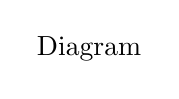
\begin{tikzpicture}
            \node {Diagram};
        \end{tikzpicture}
    \end{center}
\end{enumerate}
